\section{Описание}
Булев поиск представляет собой метод поиска документов по запросам, составленным из терминов и логических операторов AND, OR с возможностью группировки с помощью скобок. В данной работе реализован механизм выполнения булевых запросов на основе ранее построенного инвертированного индекса. Система преобразует запрос в инфиксной нотации (привычной нам) в обратную польскую нотацию (RPN) и вычисляет результат с использованием стека и операций над отсортированными списками ID документов. \\

\vspace{1 em}
\noindent\textbf{Формат представления поискового запроса.} Формат -- это привычная нам запись логических выражений с бинарными операторами AND и OR и круглыми скобками для задания приоритета. Примеры запросов:
\begin{itemize}
    \item \texttt{apple AND orange}
    \item \texttt{apple OR banana}
    \item \texttt{(apple OR banana) AND orange}
\end{itemize}
\pagebreak

\section{Исходный код}

\vspace{1 em}
\noindent\textbf{Алгоритм выполнения булева запроса.}

\begin{enumerate}
    \item \textbf{Токенизация запроса:} Исходная строка запроса разбивается на токены: термины, операторы AND, OR, скобки. Процесс игнорирует пробельные символы и учитывает регистр только для терминов (операторы не чувствительны к регистру). Проводится нормализация токенов и стемминг (при помощи ранее разработанных нами библиотек \texttt{normalizer\_lib.c} и \texttt{stemmer\_lib.c}).
    \item \textbf{Преобразование в обратную польскую нотацию.} Запрос преобразуется в RPN (этот формат удобнее использовать компьютеру при разборе логических выражений) с использованием алгоритма сортировочной станции (Shunting-yard). Алгоритм использует выходную очередь и стек операторов. Приоритет операторов: AND выше чем операторов OR. Скобки изменяют стандартный порядок обработки. Результатом является последовательность токенов в RPN, где операторы следуют за своими операндами.
    \item \textbf{Вычисление RPN выражения.} Вычисление производится с помощью списков ID документов. Алгоритм последовательно обрабатывает токены RPN:
    \begin{itemize}
        \item Если токен — термин, загружается соответствующий ему постлист из индекса (с использованием хэш-таблицы для быстрого поиска) и помещается в стек.
        \item Если токен — бинарный оператор (AND или OR), из стека извлекаются два верхних списка, выполняется соответствующая операция, результат помещается обратно в стек.
    \end{itemize}
    После обработки всех токенов в стеке остается один список — результат выполнения всего запроса.
\end{enumerate}

\vspace{1 em}
\noindent\textbf{Алгоритмы выполнения базовых операций.} Они основаны на методе слияния, аналогичном используемому в сортировке слиянием. Оба алгоритма требуют, чтобы входные списки были отсортированы по возрастанию ID документов (что верно для построенного индекса).

\begin{itemize}
    \item \textbf{Пересечение (AND).} Алгоритм строит список документов, содержащих оба термина. Используются два указателя, изначально установленные на начала списков. На каждом шаге сравниваются текущие элементы. Если ID равны, элемент добавляется в результат, и оба указателя сдвигаются. Если ID в первом списке меньше, сдвигается указатель первого списка, иначе -- второго. Сложность алгоритма -- O(n + m), где n и m — длины списков.
    
    \item \textbf{Объединение (OR).} Алгоритм строит список документов, содержащих хотя бы один из терминов. Используется метод слияния с двумя указателями. На каждом шаге в результат добавляется меньший из текущих элементов, и сдвигается соответствующий указатель. При равенстве ID элемент добавляется один раз, и сдвигаются оба указателя. Сложность алгоритма -- O(n + m).
\end{itemize}

\begin{lstlisting}[language=C]
uint32_t * intersect_lists( uint32_t * list1, uint32_t count1,
                            uint32_t * list2, uint32_t count2,
                            uint32_t * result_count )
{
    if ( count1 == 0 || count2 == 0 )
    {
        *result_count = 0;
        return NULL;
    }
    
    if ( count1 > count2 )
    {
        uint32_t * temp_list = list1;
        uint32_t temp_count = count1;
        list1 = list2;
        count1 = count2;
        list2 = temp_list;
        count2 = temp_count;
    }
    
    uint32_t * result = malloc( count1 * sizeof( uint32_t ) );
    uint32_t i = 0, j = 0, k = 0;
    
    while ( i < count1 && j < count2 )
    {
        if ( list1[i] == list2[j] )
        {
            result[k++] = list1[i];
            i++;
            j++;
        }
        else if ( list1[i] < list2[j] )
        {
            i++;
        }
        else
        {
            j++;
        }
    }
    
    *result_count = k;
    return result;
}

uint32_t * union_lists( uint32_t * list1, uint32_t count1,
                        uint32_t * list2, uint32_t count2,
                        uint32_t * result_count )
{
    uint32_t * result = malloc( ( count1 + count2 ) * sizeof( uint32_t ) );
    uint32_t i = 0, j = 0, k = 0;
    
    while ( i < count1 && j < count2 )
    {
        if ( list1[i] == list2[j] )
        {
            result[k++] = list1[i];
            i++;
            j++;
        }
        else if ( list1[i] < list2[j] )
        {
            result[k++] = list1[i];
            i++;
        }
        else
        {
            result[k++] = list2[j];
            j++;
        }
    }
    
    while ( i < count1 )
    {
        result[k++] = list1[i++];
    }
    
    while ( j < count2 )
    {
        result[k++] = list2[j++];
    }
    
    *result_count = k;
    return result;
}
\end{lstlisting}

\vspace{1 em}
\noindent\textbf{Стратегия оптимизации порядка выполнения операций.} В рамках алгоритмов пересечения и объединения реализована эвристика для операции AND: при пересечении двух списков более короткий список всегда помещается первым аргументом, что может незначительно ускорить обработку за счет более раннего завершения при наличии очень короткого списка.

\vspace{1 em}
\noindent\textbf{Поиск термина в загруженном индексе.} Изначально термин ищется в индексе через хэш-таблицу. При загрузке индекса в память строится хэш-таблица, в которую помещаются все термины словаря вместе с метаданными (смещение постлиста в файле и количество документов). Коллизии разрешаются методом цепочек. Это обеспечивает амортизированное время поиска. Заметим, что бинарный поиск мог бы быть применен к отсортированному массиву терминов, загруженному в память, что дало бы гарантированное время поиска O(log N) и потребовало бы меньше памяти (считаем скорость выполнения запроса приоритетной).

\vspace{1 em}
\noindent\textbf{Пример.} Использование полученной утилиты:

        printf( "  Построение индекса: %s <директория_с_файлами>\n", argv[0] );
        printf( "  Поиск по индексу: %s -search <термин>\n", argv[0] );
        printf( "  Булев поиск: %s -bool \"запрос\"\n", argv[0] );

\begin{enumerate}
    \item \textbf{./indexer <in\_dir>} –- построение индекса из корпуса, находящегося в указанной директории
    \item \textbf{./indexer -search <термин>} -- вывод ID документов, содержащих указанный термин
    \item \textbf{./indexer -bool <запрос>} -- выполнение бинарного поиска по указанному запросу
\end{enumerate}

Результаты выполнения запроса соответсвуют статьям об игре Marvel Rivals, которая действительно считается клоном проекта Overwatch.

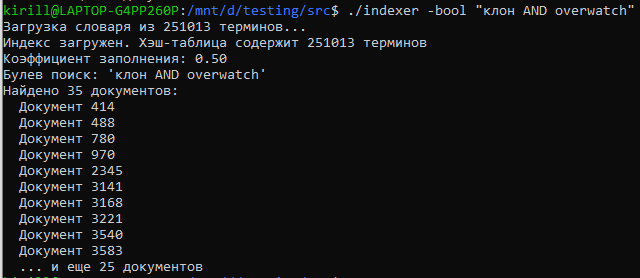
\includegraphics[width=\textwidth, height=\textheight, keepaspectratio]{pics/example.png}

\vspace{2em}
\noindent\textbf{Документ 414.}
\begin{tcolorbox}[colback=blue!5!white,colframe=blue!75!black]
Marvel Rivals: Превью самого удачного клона Overwatch Супергерои не умирают Алексей Лихачев По вселенной Marvel что только не выходило: и файтинги ( Marvel vs. Capcom), и пошаговая тактика ( Marvel’s Midnight Suns), и карточная игра ( Marvel Snap), и многочисленные мобильные развлечения. Но никто не брался за геройский шутер, хотя с таким количеством персонажей он рано или поздно должен был появиться. Успех Overwatch вдохновил многих разработчиков — оказалось, героям в таких играх необязательно носить с собой пушки и стрелять. И Marvel Rivals чуть ли не целиком копирует формулу Overwatch — зачастую такая характеристика используется в негативном ключе, но в данном случае писать об игре что-то плохое не хочется. Что-то знакомоеЗаимствования встречаются на каждом шагу. В командах здесь по шесть игроков, как в первой Overwatch. .....
\end{tcolorbox}

\pagebreak

